\section*{Implementation}

FALDO is a small OWL2 ontology with 14 classes of which 9 deal with the concept of a position on a sequence (Figure \ref{fig:ontology}).
Four of those classes are used to describe accurately what we know of a position that is not precisely determined.
Four classes are used to describe the concept of a position on a strand of DNA, e.g. positive, negative and on both strands.
All eight of these classes are sub classes of the generic $\mathtt{faldo\colon{}Position}$ super-class.
The ninth class is the concept of a region i.e. something with an end and start position.
In contrast to other representations, FALDO has no explicit way to say that it is not ``known'' on which strand a position is, because this explicit statement unknown strand position can introduce contradictions when merging different data sets.
For example, some positions could end up being contradictorily typed both as forward-stranded as well as being located on an unknown strand position.

There are 3 more classes ($\mathtt{faldo\colon{}CollectionOfRegions}$ and its subclasses) that are only there for backwards compatibility with INSDC join features with uncertain semantics. i.e. those join regions where a conversion program can only state that there are some regions and that the order that they are declared in the INSDC record might have biological significance.
However, here the INSDC record needs intelligent inspection before the data can be cleanly converted to a data model with rich semantics.

FALDO defines a single datatype property,
$\mathtt{faldo\colon{}position}$, that is used to provide a one-based
integer offset from the start of a reference sequence.
This property, when used together with the
$\mathtt{faldo\colon{}reference}$ property, links the concept of
a $\mathtt{faldo\colon{}Position}$ to an instance of a biological
sequence.
Note that these terms are case-sensitive:
$\mathtt{faldo\colon{}position}$ is a property, and
$\mathtt{faldo\colon{}Position}$ is a concept.

For compatibility with a wide range of data, FALDO makes very few
assumptions about the representation of the reference sequence, and
can be used to describe positions on both single- and double-stranded
sequences.
When both strands of a double-stranded sequence are represented by a
single entity (recommended over each strand being represented
separately), integer $\mathtt{faldo\colon{}position}$ properties are
counted from the 5' end of whichever strand is considered the
``forward'' strand.

A key part of the FALDO model is the separation of feature and where a feature is found in a sequence record.
For this we use the $\mathtt{faldo\colon{}location}$ object property. 
This property is used to distinguish between a conceptual gene as an ``unit of inheritance'' and the corresponding representation of the DNA sequence region encoding the gene as stored in a database.

As in the INSDC data model and the associated GenBank ASN.1 notation,
each location in FALDO has an identifier for the sequence it is found on \cite{NCBI}.
This means that the position information is complete without further references to the context the position information was found in.
The difference is that in FALDO, due to its RDF nature, the identifier of the sequence is a dereferencable pointer (URI) on the web, instead of just a string of characters.


\begin{figure}
\begin{center}
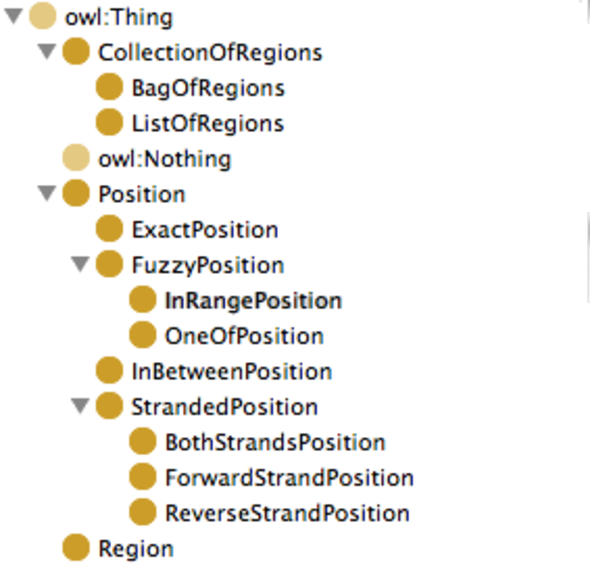
\includegraphics[height=10cm]{figures/classes.pdf}
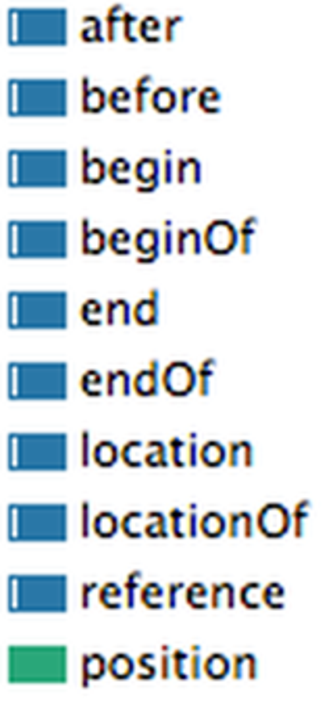
\includegraphics[width=3.5cm]{figures/properties.pdf}
\end{center}
\caption{The classes and object properties used in FALDO}
\label{fig:ontology}
\end{figure}


\begin{figure}
\begin{center}
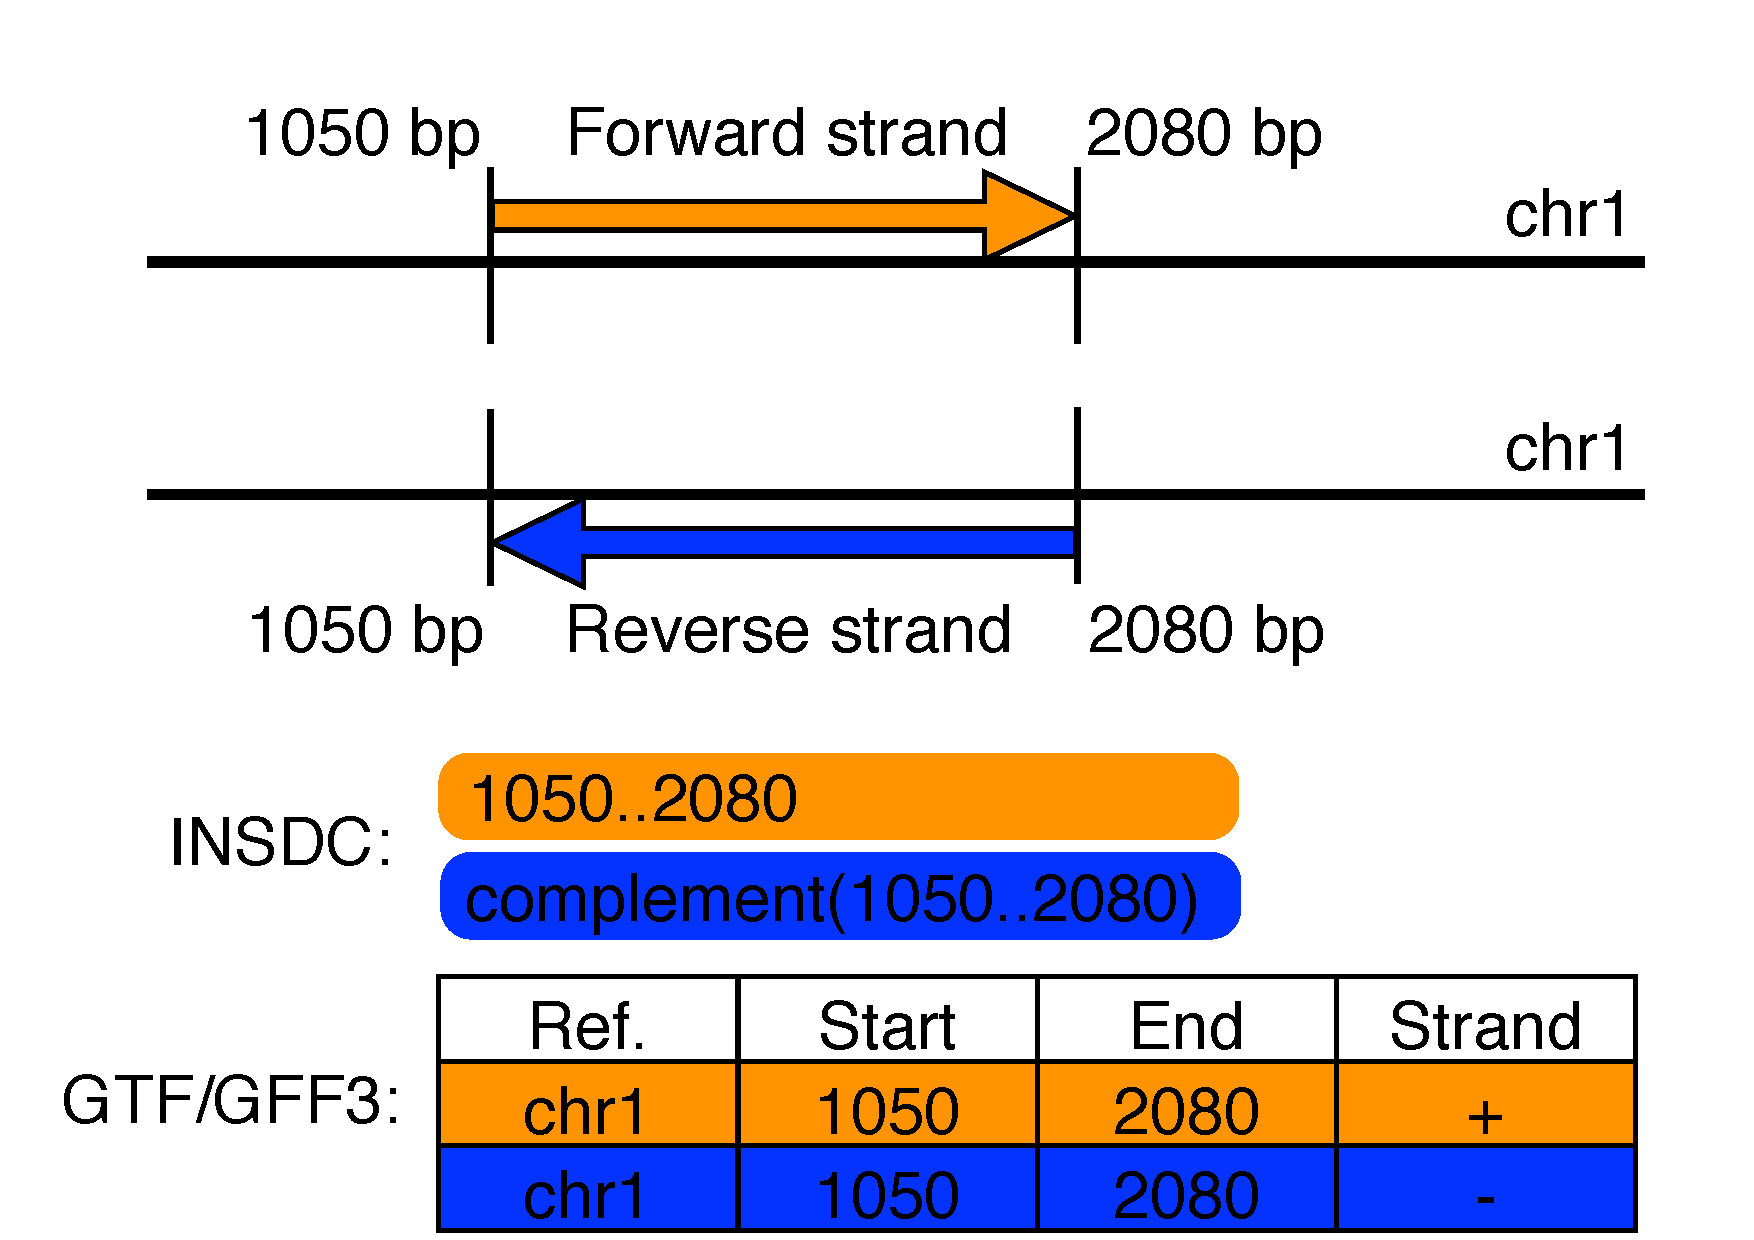
\includegraphics[width=8cm]{figures/figures.pdf}
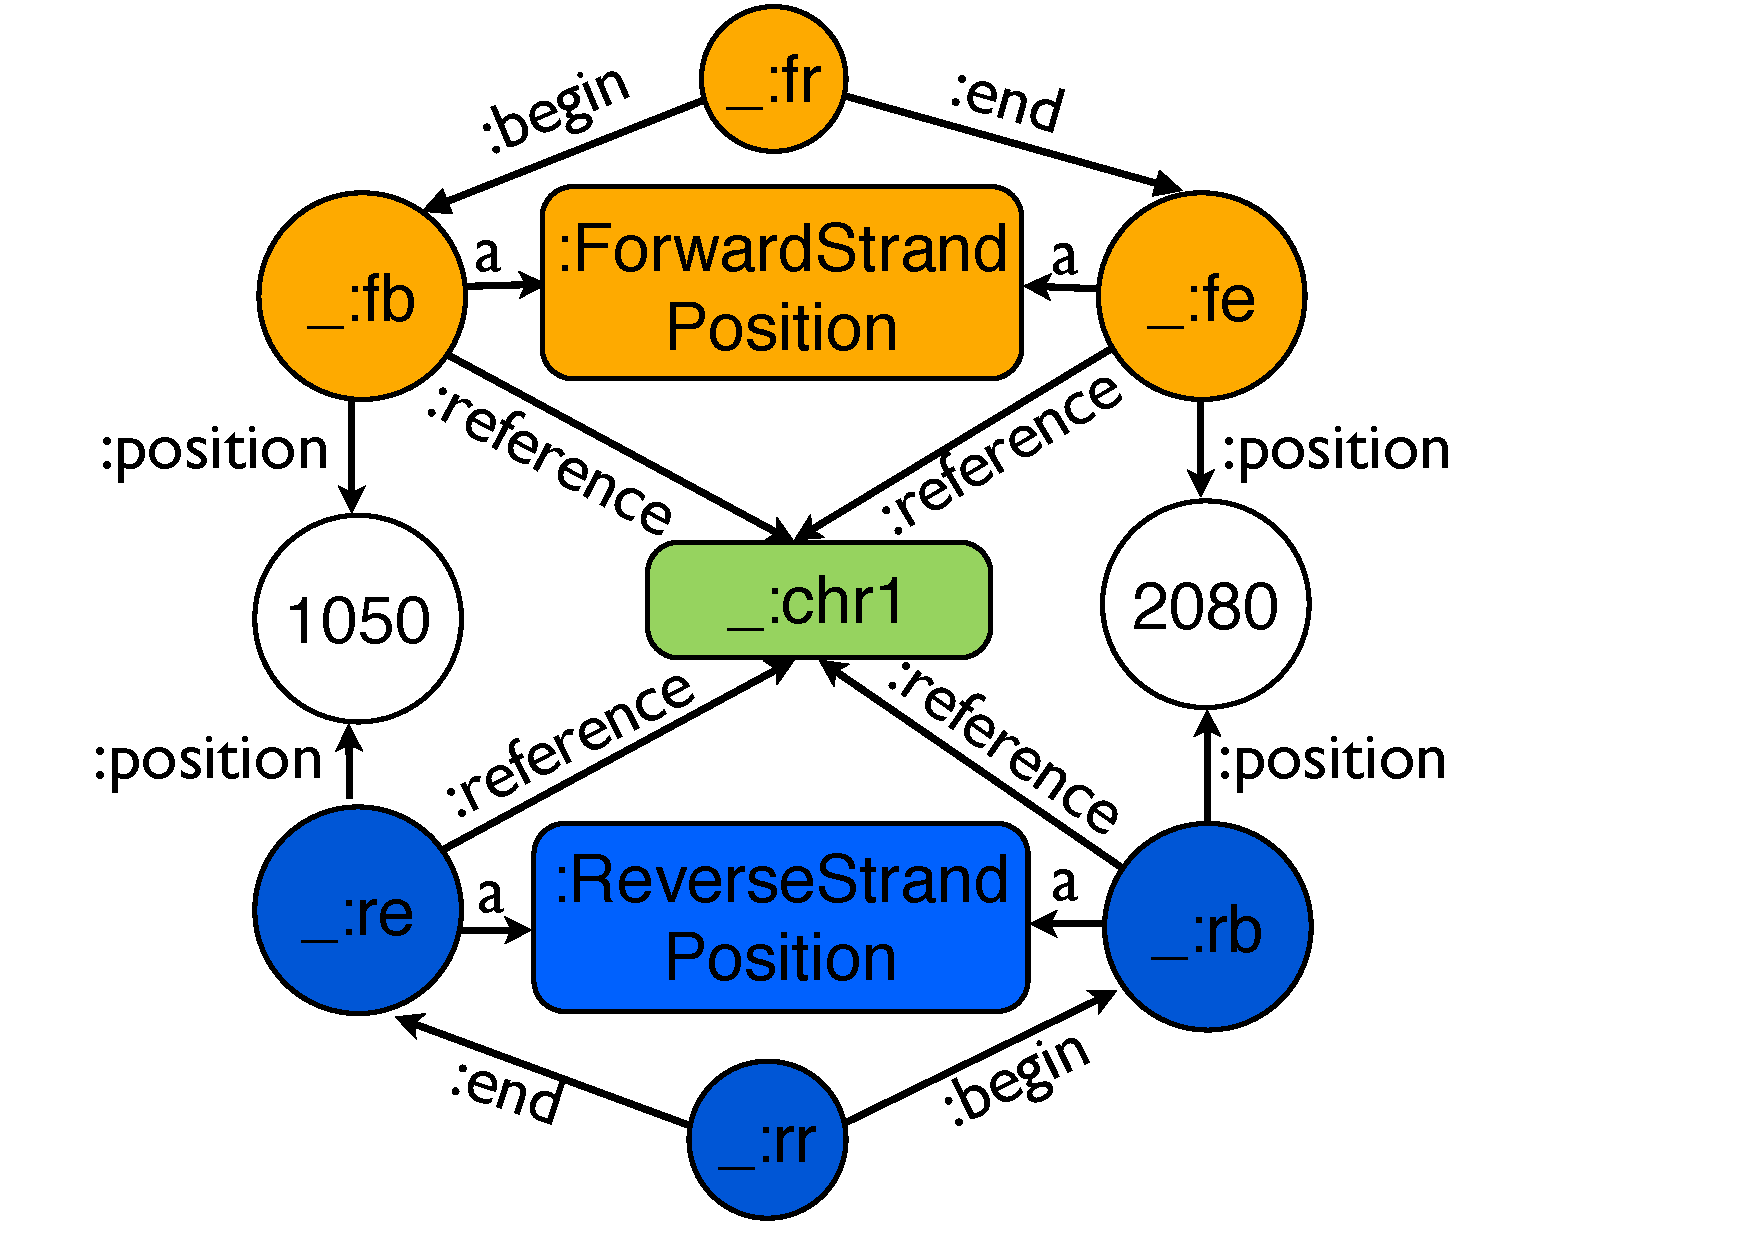
\includegraphics[width=8cm]{figures/figures3.pdf}
\end{center}
\caption{Assorted conventions for regions, start, end, and strands.
This figure shows two hypothetical features on a DNA sequence
(labeled \texttt{chr1}), on either the forward strand (orange) or
reverse strand (blue).
Using the INSDC location string notation, these regions are
``\texttt{1050..2080}'' and ``\texttt{complement(1050..2080)}''
respectively if implicitly given in terms of the reference chr1.
Using the GTF/GFF3 family of formats, regardless of the
strand these two locations are described with $start = 1050$
and $end = 2080$, and in general, $start \leq end$.
Biologically speaking, in terms of transcription, the start of a genomic
feature is strand dependent.
For the forward strand feature (orange), the start is 1050
while the reverse strand feature (blue) starts from 2080.}
\label{fig:strands}
\end{figure}

\subsection*{Compression via OWL2 reasoning}
For large databases such as INSDC or UniProt,
the need to repeat the reference sequence for each position may come with a significant cost in storage.
However, this triple does not need to be materialised in the database, as it is inferrable using OWL2 property chain reasoning.
With the axiom shown in Figure~\ref{owl:chainProperty} the $\mathtt{faldo\colon{}reference}$ triples can be inferred for any $\mathtt{faldo\colon{}position}$ described by an INSDC record.
Having an OWL-capable query rewriter allows users to ignore the difference between encoding the $\mathtt{faldo\colon{}reference}$ properties explicitly and having them inferred at query time.
For RDF databases that do not offer this capability,
the necessary triples can be easily added using a single SPARQL insert query (Figure~\ref{sparql:chainProperty}).
This flexibility allows users of the data to select the best approach for their infrastructure, rather than being constrained by the decisions of the data provider.

\begin{figure}
\begin{shaded}
\small
\begin{verbatim}
insdc:reference
      a       owl:ObjectProperty ;
      rdfs:subPropertyOf faldo:reference ;
      owl:propertyChainAxiom
              (faldo:endOf faldo:locationOf insdc:featureOf insdc:sequence) , 
              (faldo:locationOf insdc:featureOf insdc:sequence) , 
              (faldo:beginOf faldo:locationOf insdc:featureOf insdc:sequence) .

\end{verbatim}
\end{shaded}
\caption{OWL2 property chain axiom to infer that all positions described in an INSDC record are relative to the main sequence of the record (in RDF turtle syntax, prefixes ommited).}
\label{owl:chainProperty}
\end{figure}

\begin{figure}
\begin{shaded}
\small
\begin{verbatim}
INSERT {
    ?position faldo:reference ?sequence .
}
WHERE {
    ?record a insdc:Entry ;
            insdc:feature ?feature ;
            insdc:sequence ?sequence .
    ?feature faldo:location ?location .
      { ?location faldo:begin|faldo:end ?position . }
    UNION
      { ?location a faldo:Position . }
}
\end{verbatim}
\end{shaded}
\caption{A SPARQL query to add all $\mathtt{faldo\colon{}reference}$ properties to $\mathtt{faldo\colon{}positions}$ described from a $\mathtt{insdc\colon{}record}$.}
\label{sparql:chainProperty}
\end{figure}

\subsection*{Validating data encoded with FALDO}

Some databases only allow a subset of FALDO. 
For example INSDC requires that the start and end of a region are on the same sequence,
while UniProt requires that a feature is described in relation to the reference's canonical isoform.
Yet another database might annotate the location of a glycsoylation site on an UniProt isoform sequence.
When added to an UniProt record in RDF, this extra RDF annotation would be ignored by applications that are not concerned with glycosylation of isoforms.
The same annotation can not be added to UniProt XML as the XSD schema does not allow for it,
and the older plain text flat-file format does not allow for this kind of third party extension either.
An attempt to add such information would very likely break any XML or flat-file parser and introduces the risk of importing data incorrectly.
Only the UniProt RDF format allows other people to make assertions about UniProt data without breaking existing tools.

There are many ways to add constraints to the data model by applications using Semantic Web technologies\cite{RDFValidationReport}.
In other words, data validation is an application specific concern instead of a data format concern.

\subsection*{Users}
FALDO is already deployed and used in a number of tools and databases.

\begin{description}
\item[JBrowse] can use SPARQL queries with FALDO to visualize annotations on reference sequences from semantic databases \cite{JBrowse}.
\item[INSDC-DDBJ] DDBJ is currently working on an RDF format for the INSDC data that is stored in DDBJ/GenBank/EMBL-Bank.
\item[BioInterchange] uses FALDO to make position information in current bioinformatics data stored in GFF3-, GVF-, GTF-, or VCF-files available to the semantic web (\url{http://www.biointerchange.org/}).
\item[TogoGenome] a genome database collection provided by the DBCLS also uses FALDO in its RDF representation (\url{http://togogenome.org/}).
\item[InterMine] The popular model organism database software collection uses FALDO in its SPARQL mode \cite{InterMine}.
\item[PhenomeBrowser] Positions of phenotypes and disease related natural variations are positioned onto the mouse genome using FALDO.
\item[BOING] The ``bio-ontology integrated querying of sequence annotations'' framework uses FALDO to describe all feature locations \cite{BOING}.
\item[SPARQL-BED] This simple tool that turns any BED file into a Web accessible SPARQL endpoint using FALDO to describe BED feature positions (\url{https://github.com/JervenBolleman/sparql-bed}).
\item[BioPerl] BioPerl\cite{BioPerl2002} now includes a FALDO exporter (\texttt{Bio::FeatureIO::faldo}), which allows any BioPerl-supported feature format to be translated to FALDO.
\item[UniProt] UniProt annotates many protein features and sites. Starting with UniProt RDF release 2014$\_$01 the positions of protein feature are described using FALDO.
\end{description}

